\documentclass{beamer}
 
\usepackage[utf8]{inputenc}
\usepackage{amsfonts, amssymb, amsmath}    
\usepackage{graphicx}
\graphicspath{ {images/} }
\usetheme{Berkeley}
\usecolortheme{seahorse}

\newcommand{\bX}{\mathbf{X}}
\newcommand{\bY}{\mathbf{Y}}
\newcommand{\bbeta}{\mathbf{\beta}}
 
\title[Survival of the Fittest]
{Survival of the Fittest: Variable Selection on Agricultural Data from the Gal\'apagos Islands}

\author
{Michael Bostwick}

 
\date
{April 19th, 2018}
 
 
 
\begin{document}
 
\frame{\titlepage}

\begin{frame}
\frametitle{Table of Contents}
\tableofcontents
\end{frame}
 
\section{Background}

\begin{frame}
\frametitle{Gal\'apagos Islands}
\end{frame}

\begin{frame}
\frametitle{Agent-Based Simulation}
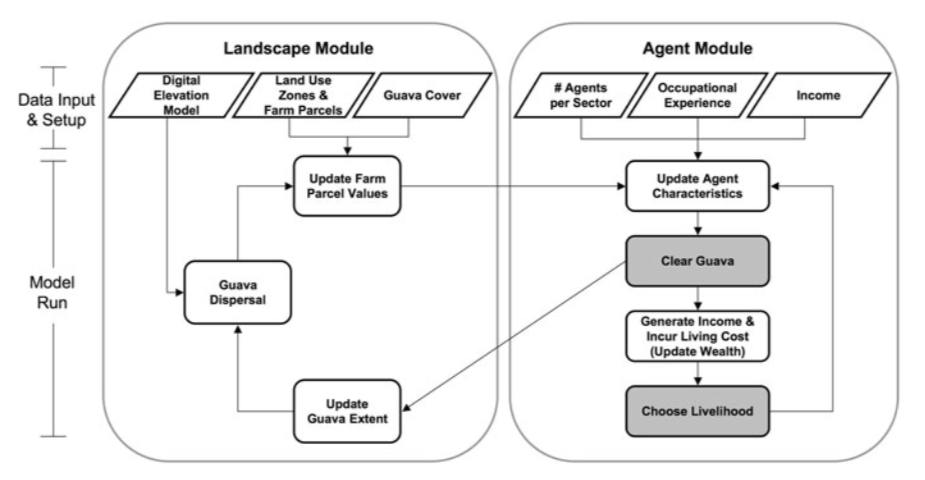
\includegraphics[scale=0.3]{abm_chart}

From Miller et. al.

\end{frame}

\section{Data}

\begin{frame}
\frametitle{Data description}
\end{frame}

\begin{frame}
\frametitle{Data transformation}
\end{frame}

\section{Modeling}

\begin{frame}
\frametitle{Elastic Net}

\begin{block}{Formulation}
	\[\min_{\beta}  \|\bY - \bX\beta\|_{2}^{2} + \lambda[ \underbrace{(1 - \alpha)||\beta||_2^2}_\text{Ridge} + \underbrace{\alpha||\beta||}_\text{LASSO}]\]
\end{block}

\begin{itemize}
	\item{Set $\alpha$ and $\lambda$ using cross-validation}
\end{itemize} 

\end{frame}

\begin{frame}
\frametitle{Forward Stepwise}
\end{frame}

\section{Results}

\begin{frame}
\frametitle{Productivity Model - Elastic Net}
\end{frame}

\begin{frame}
\frametitle{Productivity Model - Forward Stepwise}
\end{frame}

\begin{frame}
\frametitle{Productivity Model - Comparison}
\end{frame}
 
\begin{frame}
\frametitle{References}

\end{frame}
\end{document}